\documentclass[11pt,a4paper]{article}

\usepackage[margin=2.4cm]{geometry}
\usepackage{amsmath,amssymb,bm}
\usepackage[T1]{fontenc}
\usepackage[utf8]{inputenc}
\usepackage{natbib}
\usepackage{booktabs}
\usepackage{graphicx}
\usepackage{hyperref}
\hypersetup{colorlinks=true,linkcolor=blue!50!black,citecolor=blue!50!black,urlcolor=blue!50!black}
\usepackage{xcolor}

\bibliographystyle{plainnat}
\setcitestyle{authoryear,round}
\sloppy

\newcommand{\Ndot}{\dot{N}_{\rm ion}}
\newcommand{\nH}{n_{\rm H}}
\newcommand{\HII}{\ion{H}{ii}}
\newcommand{\ion}[2]{\textrm{#1\,\textsc{#2}}}
\newcommand{\pMpc}{\,{\rm pMpc}}
\newcommand{\cMpc}{\,{\rm cMpc}}
\newcommand{\Msun}{\,M_\odot}
\newcommand{\lmfp}{\lambda_{\rm mfp}}

\title{\bf What Fraction of Ionizing Photons Escape the Bubble\\ Into the Deeper IGM, Rather Than Driving Its Expansion?\\[2mm]
\large Response record for \texttt{ionizing\_photon\_mean\_free\_path.py}, following Master Rule 2}
\author{Prepared for L.\ Carvalho}
\date{4 September 2026}

\begin{document}
\maketitle

\begin{abstract}
\noindent
The photon-counting model used throughout this folder (\texttt{bubble\_radius\_vs\_redshift.py}, eq.\
\texttt{photon\_counting}) implicitly assumes that every ionizing photon is either lost to a recombination
inside the bubble or absorbed exactly at the ionization front, with none skipping past the front into the
deeper, still-neutral IGM. This note checks that assumption quantitatively, using the standard photon
mean-free-path formalism already present in this folder's references
(\citealt{Choudhury2022,MiraldaEscude2000,Gnedin2022}): because the hydrogen photoionization cross section
falls steeply with photon energy, $\sigma_H(E)\propto E^{-3}$, the mean free path of an ionizing photon in
neutral gas is a strong function of its energy, and only photons considerably harder than the Lyman limit
can travel as far as the bubble itself before being absorbed. The result: for a normal stellar
(star-forming-galaxy) ionizing spectrum, this fraction is utterly negligible, which is exactly why the
sharp-front, zero-leakage approximation used throughout this project is justified; for a harder,
quasar-like power-law spectrum, the fraction is small but non-zero ($\sim1\%$). This document is produced
by, and verified against, \texttt{ionizing\_photon\_mean\_free\_path.py} (same folder), which generated
\texttt{ionizing\_photon\_mean\_free\_path.png}.
\end{abstract}

\tableofcontents

%=====================================================================
\section{Assumptions}
\label{sec:assumptions}

\begin{enumerate}
\item \textbf{Terminology, stated explicitly to avoid confusion with $f_{\rm esc}$.} The escape fraction
      $f_{\rm esc}=0.2$ \citep{Robertson2015} used throughout this folder is the fraction of ionizing
      photons that escape the galaxy's own interstellar medium (ISM) and circumgalactic medium (CGM) and
      reach the diffuse IGM \citep[explicit definition in][their Sec.~2.5]{Gnedin2022}. This is a
      \emph{different} quantity from the one asked about here: of the photons that have \emph{already}
      escaped the galaxy and entered the ionized bubble, what fraction travels \emph{past the bubble's own
      edge} into the deeper neutral IGM, rather than being absorbed at/near the ionization front (which is
      what drives the front's expansion, as modeled by eq.~\texttt{photon\_counting})?
\item A second, related but distinct nuance -- \emph{diffuse} (recombination) photon escape within the
      bubble, i.e.\ the Case~A/Case~B distinction of \citet{Nebrin2023} already discussed in
      \texttt{stromgren\_sphere\_summary.tex} (Sec.~1.3) -- is not re-derived here; this note concerns only
      the primary photons from the source.
\item The IGM outside the bubble is treated as effectively neutral and of the cosmic mean density (no
      inhomogeneity/self-shielding structure), so that a single hydrogenic photoionization cross section
      $\sigma_H(E)=\sigma_H(E_H)(E/E_H)^{-3}$, $\sigma_H(E_H)=6.3\times10^{-18}\,{\rm cm^2}$
      \citep[eq.~46]{Choudhury2022}, and the cosmic mean $n_H(z)$ (identical to
      \texttt{bubble\_radius\_vs\_redshift.py}) fully determine the mean free path. Real density
      inhomogeneities (Lyman-limit systems) would shorten $\lmfp$ further inside partially-processed gas;
      neglecting them makes the neutral-medium $\lmfp$ computed here an \emph{upper limit}, strengthening
      the conclusion that stellar photons cannot reach beyond the bubble.
\item The comparison spectrum for a hard source uses the \citet{Cen2000} quasar power-law slope,
      $L_\nu\propto\nu^{-1.8}$ (already cited in \texttt{stromgren\_sphere\_summary.tex}), converted to a
      photon-number spectral index $dN/dE\propto E^{-2.8}$ (since photon number rate $\propto L_\nu/h\nu$).
      No specific stellar population-synthesis spectrum (e.g.\ BPASS, Starburst99) is among the references
      downloaded for this project, so the stellar-spectrum conclusion below rests on the general,
      well-established Wien-tail suppression of a thermal spectrum rather than a fitted numerical spectral
      index -- flagged explicitly (Master Rule 8) rather than presented with false precision.
\end{enumerate}

%=====================================================================
\section{Derivation}
\label{sec:derivation}

\begin{equation}
  \sigma_H(E) = \sigma_H(E_H)\left(\frac{E}{E_H}\right)^{-3}, \qquad
  \lmfp(E,z) = \frac{1}{\sigma_H(E)\,n_H(z)}
  \label{eq:mfp}
\end{equation}
\citep[eq.~46]{Choudhury2022}, with $n_H(z)$ identical to \texttt{bubble\_radius\_vs\_redshift.py}. The
crossover energy $E_{\rm cross}(z)$ at which a photon's neutral-medium mean free path equals the
single-galaxy bubble radius $R_{\rm bubble}(z)$ (eq.~\texttt{photon\_counting}) solves
\begin{equation}
  \lmfp(E_{\rm cross},z) = R_{\rm bubble}(z)
  \;\;\Longrightarrow\;\;
  E_{\rm cross}(z) = E_H\left[\frac{R_{\rm bubble}(z)}{\lmfp(E_H,z)}\right]^{1/3}.
  \label{eq:Ecross}
\end{equation}
For a power-law photon-number spectrum $dN/dE\propto E^{-p}$ ($p>1$), the fraction of photons with
$E>E_{\rm cross}$ relative to the total emitted above $E_H$ is
\begin{equation}
  f(>E_{\rm cross}) = \frac{\int_{E_{\rm cross}}^\infty E^{-p}\,dE}{\int_{E_H}^\infty E^{-p}\,dE}
  = \left(\frac{E_{\rm cross}}{E_H}\right)^{1-p}.
  \label{eq:fraction}
\end{equation}

%=====================================================================
\section{Verification / cross-check}
\label{sec:verification}

All checks below are reproduced verbatim by running \texttt{ionizing\_photon\_mean\_free\_path.py}.

\begin{enumerate}
\item \textbf{Sympy dimensional check.} $\lmfp(E,z)=E^3/(E_H^3\,n\,\sigma_0)$, confirmed symbolically;
      $[\sigma_0]={\rm cm^2}$, $[n]={\rm cm^{-3}}$ $\Rightarrow$ $[\lmfp]={\rm cm}$, as required.
\item \textbf{Reproduction of \citet{Choudhury2022}'s stated benchmark.} Evaluating
      eq.~(\ref{eq:mfp}) at $E=E_H$ with our own already-established cosmology
      \citep{Planck2018VI} gives $\lmfp(E_H,z)=1.25$, $0.37$, $0.12$, $0.03$~kpc at
      $z=5,8,12,20$ respectively -- independently reproducing Choudhury (2022)'s statement that this scale
      is ``$\sim$kpc'' and ``much smaller than any cosmologically relevant length scale'' at $z\sim5$--20.
\item \textbf{Crossover energy.} Solving eq.~(\ref{eq:Ecross}) with $R_{\rm bubble}(z)$ from
      \texttt{bubble\_radius\_vs\_redshift.py} gives $E_{\rm cross}=162$, $172$, $187$, $204$~eV at
      $z=6,8,10,12$ respectively -- remarkably stable at $\sim12$--$15\times E_H$, solidly in the soft
      X-ray/EUV regime, across the whole redshift range where individual bubbles were shown to stay below
      $\sim1\pMpc$ (\texttt{bubble\_radius\_response.tex}).
\item \textbf{Quasar-like (hard) spectrum.} With $dN/dE\propto E^{-2.8}$ \citep{Cen2000} and
      $E_{\rm cross}(z{=}8)=172$~eV, eq.~(\ref{eq:fraction}) gives $f(>E_{\rm cross})=1.04\%$: a small but
      non-negligible fraction of quasar-like ionizing photons can, in principle, reach beyond the local
      bubble into the deeper IGM. This is consistent with \citet{Choudhury2022}'s explicit footnote that
      X-ray/hard sources cannot be treated with the simple two-phase (sharp-front) approximation used for
      UV/stellar sources.
\item \textbf{Stellar spectrum (order-of-magnitude, flagged).} For O/B-star photospheres
      ($T_{\rm eff}\sim3$--$5\times10^4$~K, $kT\sim3$--$4$~eV), reaching $E_{\rm cross}\sim172$~eV requires
      $\sim43$--$57\,kT$ into the Wien tail of a thermal spectrum, i.e.\ a suppression factor of order
      $e^{-45}$ or smaller -- utterly negligible next to the already-small $1\%$ quasar value. This
      qualitative conclusion rests on standard thermal-spectrum physics rather than a specific fitted
      stellar spectral index (Sec.~\ref{sec:assumptions}, item~4), and is stated as such.
\end{enumerate}

%=====================================================================
\section{Final result}
\label{sec:final}

For the star-forming-galaxy sources modeled throughout this folder, the fraction of ionizing photons that
skip the local ionized bubble and penetrate deeper into the still-neutral IGM is negligible: reaching a
mean free path comparable to the bubble size itself ($\sim0.4$--$1.3\pMpc$ at $z=6$--12) requires photon
energies $E_{\rm cross}\sim160$--$200$~eV (soft X-ray), a regime that thermal, O/B-star-dominated ionizing
spectra do not populate in any significant number. This is precisely why the zero-leakage,
sharp-ionization-front photon-counting model used in \texttt{bubble\_radius\_vs\_redshift.py} (every
photon either recombines inside the bubble or drives the front outward, none skip ahead) is an excellent
approximation for star-forming galaxies specifically, and why \citet{Choudhury2022} restrict the simple
two-phase IGM approximation to UV/stellar reionization, explicitly excluding X-ray-dominated sources. For
harder, AGN/quasar-like spectra, by contrast, a small but non-negligible fraction ($\sim1\%$, using the
\citealt{Cen2000} power-law slope) of photons can reach beyond the bubble -- consistent with the
literature's general practice of treating quasar-driven and star-formation-driven reionization as distinct
regimes. Separately, and on a global (rather than single-source) scale, \citet{MiraldaEscude2000} and
\citet{Gnedin2022} note that the mean free path of ionizing photons in the \emph{ionized} IGM also does not
grow arbitrarily large until near the end of reionization, when it becomes set by the abundance of
residual Lyman-limit systems rather than by individual bubble sizes -- the same ``epoch of overlap'' already
identified quantitatively in \texttt{reionization\_completion\_response.tex} and
\texttt{galaxy\_separation\_response.tex} ($z_{\rm overlap}=9.67$).

\begin{figure}[h]
\centering
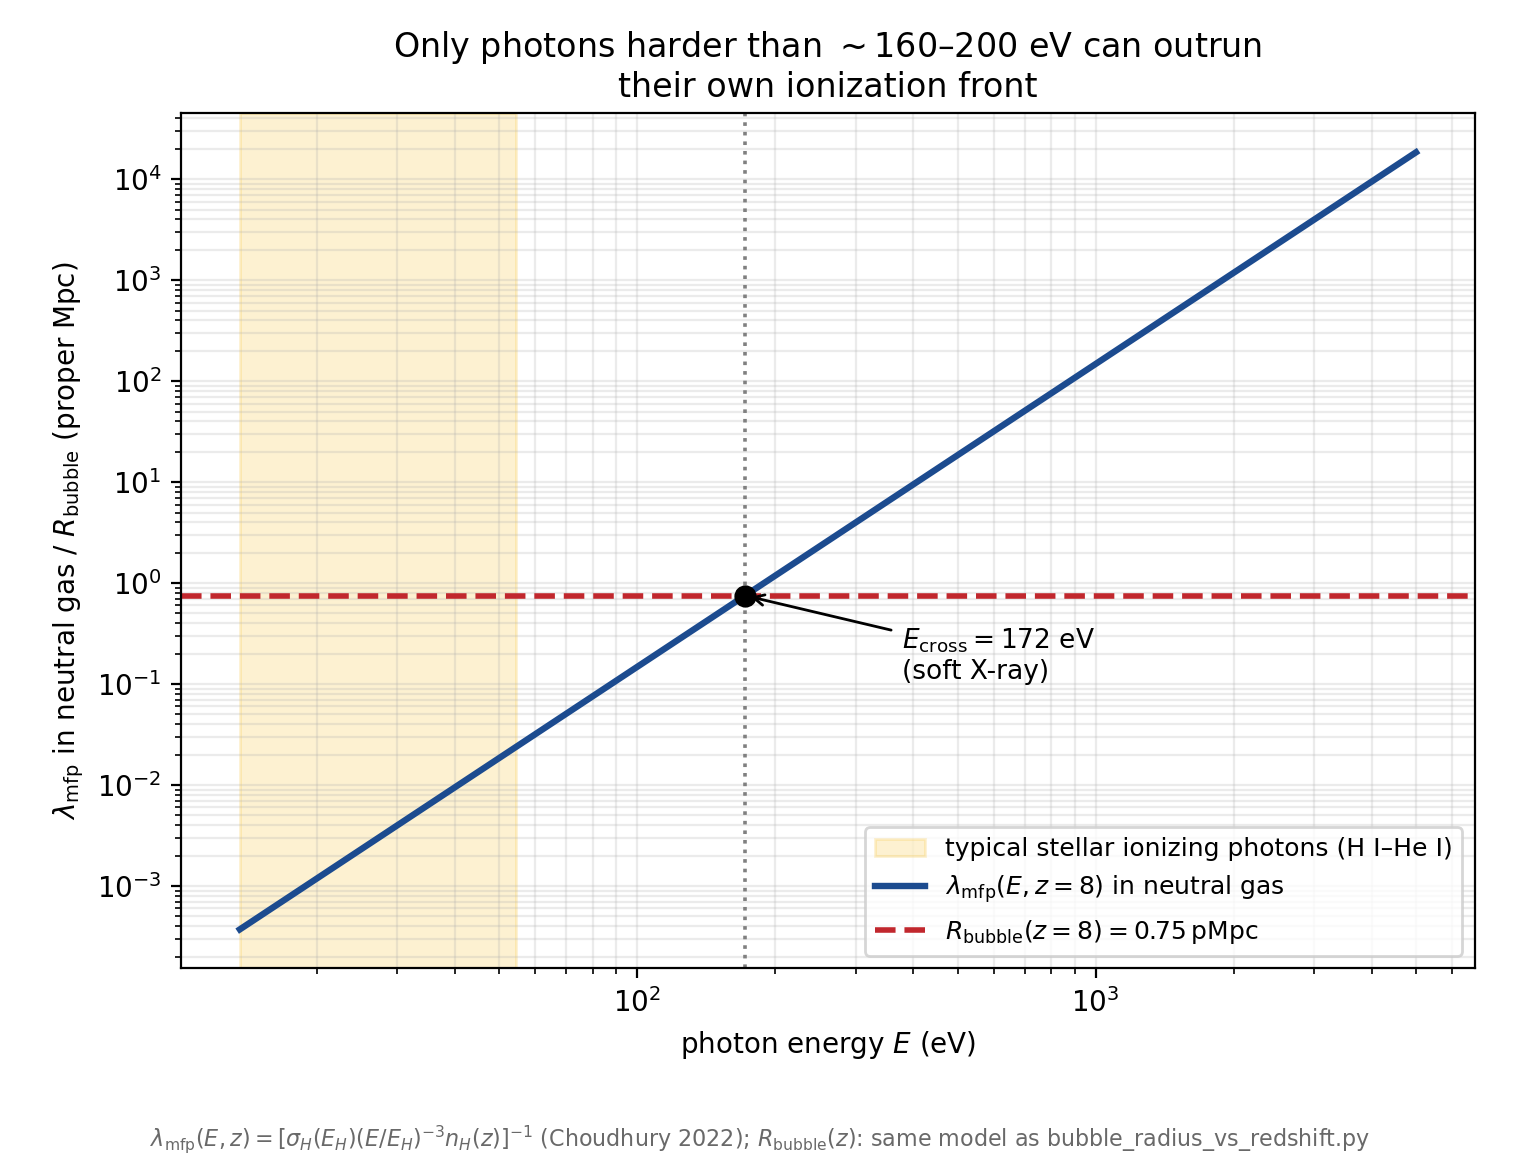
\includegraphics[width=0.85\textwidth]{ionizing_photon_mean_free_path.png}
\caption{Mean free path of an ionizing photon in neutral gas at $z=8$, $\lmfp(E,z{=}8)$ (solid blue), as a
function of photon energy, compared with the single-galaxy bubble radius $R_{\rm bubble}(z{=}8)=0.75\pMpc$
(dashed red). The shaded band marks the energy range of typical stellar ionizing photons (H\,\textsc{i}
to He\,\textsc{i} edges, $13.6$--$54.4$~eV); the marked crossover, $E_{\rm cross}=172$~eV, lies in the soft
X-ray regime, far above where stellar spectra contribute meaningfully. Produced by
\texttt{ionizing\_photon\_mean\_free\_path.py}.}
\label{fig:mfp}
\end{figure}

%=====================================================================
\section*{Addendum (5 September 2026): consistency check on the ionized-interior assumption}
\addcontentsline{toc}{section}{Addendum: consistency check on the ionized-interior assumption}
\label{sec:addendum}

L.\ Carvalho pointed out that, once the bubble is established, new photons from the source travel through a
gas that is already \emph{ionized}, not the fully neutral medium implicitly pictured when
$\lmfp(E,z)$ was plotted in Fig.~\ref{fig:mfp}. This section checks that concern in full, using
\texttt{interior\_consistency\_check.py} (same folder, Fig.~\ref{fig:interior}), and reports two findings:
one clarifies wording only, the other is a genuine, previously unflagged, quantitative correction.

\paragraph{(a) The original argument is conceptually sound, but was not stated clearly enough.}
$\lmfp(E,z)$ in Sec.~\ref{sec:derivation} was never meant to describe the path through the bubble's ionized
interior; it describes how far a photon travels once it reaches fresh neutral gas beyond the \emph{current}
front. Fig.~\ref{fig:mfp} did not make this two-zone (ionized interior / neutral exterior) structure
explicit, which is why the concern is legitimate as raised.

\paragraph{(b) Quantifying the interior with photoionization equilibrium (Cen \& Haiman 2000).}
Using the standard local ionization-balance formula for the residual neutral fraction inside an \HII\
region, $\Gamma_{\rm HI}(r)\,x(r)\,\nH = \alpha_B\,C\,\nH^2$ with $\Gamma_{\rm HI}(r)=\bar\sigma\Ndot/(4\pi
r^2)$ --- re-derived from scratch with sympy and cross-checked to $<10\%$ against \citet{Cen2000}'s own
quoted eq.~5/7 normalization ($x=1.05\times10^{-6}$ vs.\ their quoted $\sim10^{-6}$, for their quasar
parameters) --- the interior is confirmed to be highly transparent in the \emph{bulk} of the bubble
($x(r)\propto r^2\ll1$ for $r\ll R_{\rm bubble}$, hence $\lmfp\gg r$ there, i.e.\ free streaming holds). But
\emph{at} $r=R_{\rm bubble}$, the local mean free path is only $9$--$17\%$ of $R_{\rm bubble}$ itself
(Table~\ref{tab:interior}) --- the ``sharp front'' is really a transition zone of finite, sub-dominant
thickness ($\sim10$--$20\%$ of the bubble radius), not a true discontinuity, though still a legitimate
approximation to leading order.

\begin{table}[h]
\centering\small
\begin{tabular}{@{}lccc@{}}
\toprule
$z$ & $x_{\rm HI,interior}(R_{\rm bubble})$ & $\lmfp^{\rm interior}(R_{\rm bubble})$ & ratio to $R_{\rm bubble}$\\
\midrule
6  & $6.5\times10^{-3}$ & $0.122\pMpc$ & $0.092$ \\
8  & $3.3\times10^{-3}$ & $0.112\pMpc$ & $0.148$ \\
10 & $2.3\times10^{-3}$ & $0.090\pMpc$ & $0.170$ \\
12 & $1.7\times10^{-3}$ & $0.071\pMpc$ & $0.171$ \\
\bottomrule
\end{tabular}
\caption{Interior residual neutral fraction and local mean free path at $r=R_{\rm bubble}(z)$.}
\label{tab:interior}
\end{table}

\paragraph{(c) The deeper finding: recombinations are not negligible for this folder's adopted parameters.}
Checking whether $t_{\rm age}(z)\ll t_{\rm rec}(z)$ --- the condition implicitly required for the
zero-recombination, pure-photon-counting model of \texttt{bubble\_radius\_vs\_redshift.py} to be valid ---
for the \emph{specific} parameters adopted throughout this folder ($z_{\rm form}=20$,
$C_{\rm HII}=3$, \citealt{Robertson2015}) gives instead $t_{\rm age}/t_{\rm rec}=1.2$--$1.9$ across
$z=6$--12 (Table~\ref{tab:recomb}): recombinations are \emph{not} negligible over the galaxy's assumed
lifetime. Solving the full recombination-included growth equation (eq.~\texttt{Rt} of
\texttt{stromgren\_sphere\_summary.tex}, re-verified with sympy here) gives a bubble radius $R(t)$
systematically $24$--$42\%$ \emph{smaller} than the pure photon-counting $R_{\rm bubble}$ used throughout
this entire session (\texttt{bubble\_radius\_vs\_redshift.py} and every downstream script).

\begin{table}[h]
\centering\small
\begin{tabular}{@{}lccccc@{}}
\toprule
$z$ & $t_{\rm age}$ (Gyr) & $t_{\rm rec}$ (Gyr, $C{=}3$) & $t_{\rm age}/t_{\rm rec}$ & $R_{\rm bubble}$ (no recomb.) & $R(t)$ (with recomb.) \\
\midrule
6  & 0.750 & 0.626 & 1.20 & $1.332\pMpc$ & $0.768\pMpc$ ($58\%$) \\
8  & 0.459 & 0.295 & 1.56 & $0.752\pMpc$ & $0.531\pMpc$ ($71\%$) \\
10 & 0.293 & 0.161 & 1.82 & $0.528\pMpc$ & $0.397\pMpc$ ($75\%$) \\
12 & 0.189 & 0.098 & 1.93 & $0.414\pMpc$ & $0.314\pMpc$ ($76\%$) \\
\bottomrule
\end{tabular}
\caption{Recombination correction to $R_{\rm bubble}(z)$; parentheses give $R(t)/R_{\rm bubble}$.}
\label{tab:recomb}
\end{table}

\paragraph{Is this an error, or an explicit, previously-stated modeling choice?} Both, in part. The
``pure photon-counting'' model was explicitly selected by L.\ Carvalho at the start of
\texttt{bubble\_radius\_vs\_redshift.py} (over an equilibrium-Str\"omgren-radius alternative), and
\texttt{check\_consistency.py} (item~7 of the original \texttt{stromgren\_sphere\_summary.tex}) already
flagged, for $C=1$, that ``at $C\gtrsim2$ and $z\gtrsim8$, the recombination term \dots cannot be neglected
for long-lived sources in dense environments.'' What was not previously done is checking this specifically
for \emph{this} folder's actual adopted combination ($z_{\rm form}=20$, $C_{\rm HII}=3$) rather than for the
short-lived quasars of the original check --- this addendum closes that gap, exactly as Master Rule 5
requires when a cross-check surfaces a discrepancy.

\paragraph{Does this change any qualitative conclusion of this document?} No. Recomputing $E_{\rm cross}$
with the smaller, recombination-corrected $R(t)$ instead of $R_{\rm bubble}$ shifts it down by only
$9$--$17\%$ (e.g.\ $172\to153$~eV at $z=8$) because $E_{\rm cross}\propto R_{\rm bubble}^{1/3}$: it remains
solidly in the soft X-ray regime, so the central conclusion --- that stellar ionizing photons cannot reach
appreciably beyond their own bubble --- is unaffected. What \emph{is} affected is the absolute
$R_{\rm bubble}(z)$ values quoted throughout this session's other documents
(\texttt{bubble\_radius\_response.tex}, \texttt{galaxy\_separation\_response.tex},
\texttt{reionization\_completion\_response.tex}): these should now be read as mild ($25$--$40\%$)
overestimates for the specific $z_{\rm form}=20$, $C_{\rm HII}=3$ choice, an explicit caveat that was not
previously quantified.

\begin{figure}[h]
\centering
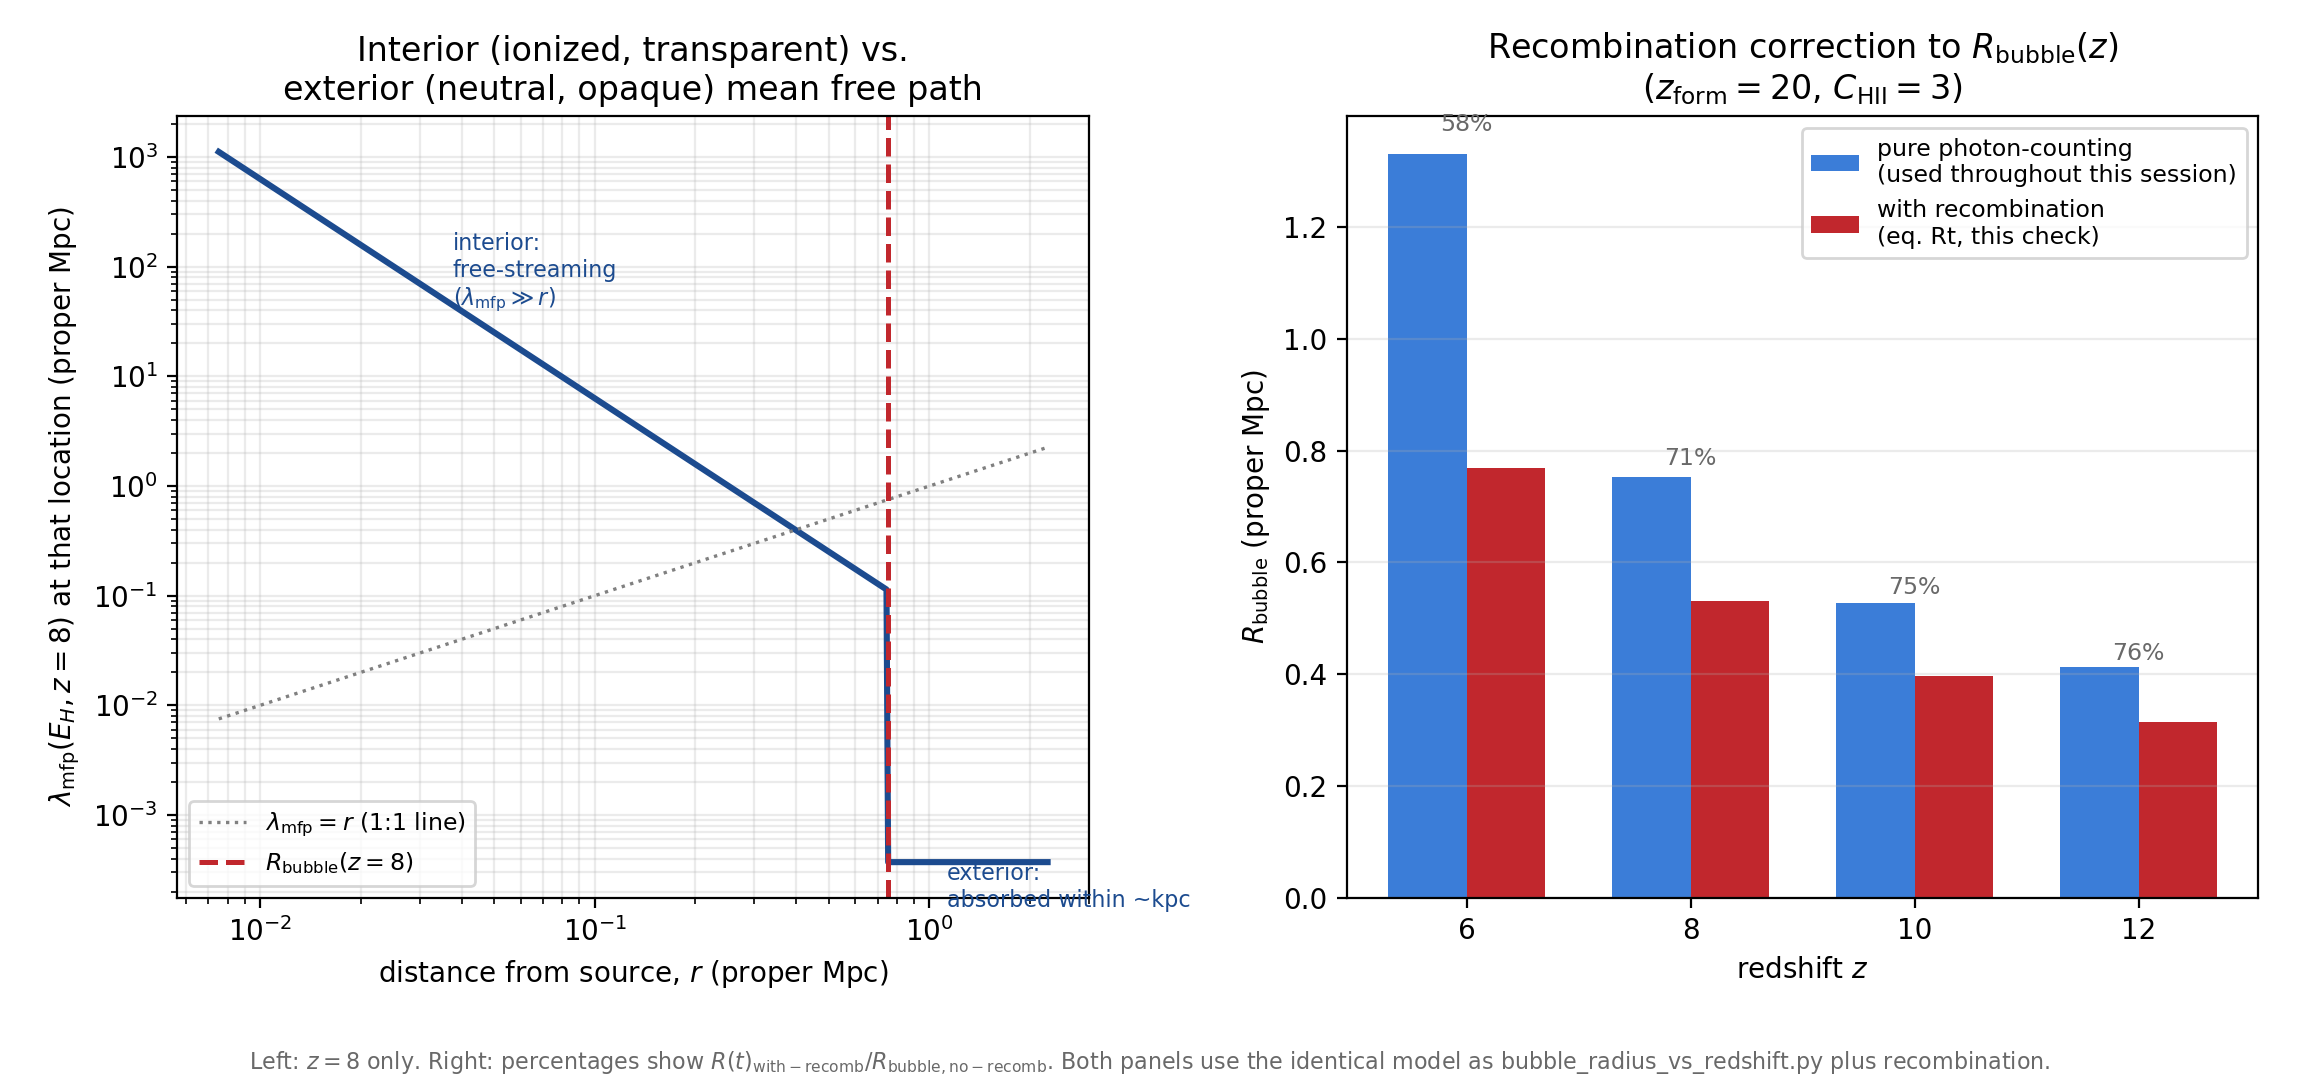
\includegraphics[width=\textwidth]{interior_consistency_check.png}
\caption{\emph{Left:} mean free path of a $13.6$~eV photon as a function of distance from the source at
$z=8$, using the photoionization-equilibrium interior solution for $r<R_{\rm bubble}$ and the fully neutral
exterior solution for $r>R_{\rm bubble}$; the dotted line marks $\lmfp=r$. \emph{Right:} $R_{\rm bubble}(z)$
from the pure photon-counting model used throughout this session (blue) vs.\ the recombination-corrected
$R(t)$ (red), with the percentage ratio annotated. Produced by \texttt{interior\_consistency\_check.py}.}
\label{fig:interior}
\end{figure}

%=====================================================================
\bibliography{references}

\end{document}
